
\documentclass{article}
\usepackage[headheight=20pt, margin=1.0in, top=1.2in]{geometry}
\usepackage{amsmath, amssymb, amsthm, thmtools, tcolorbox, array, graphicx, makeidx, cancel, multirow, fancyhdr, xypic, color, nicefrac, rotating, multicol, caption, subcaption, xcolor, tikz, tikz-3dplot, tikz-cd, pgfplots, import, enumitem, calc, booktabs, wrapfig, siunitx, hyperref,float}
\hypersetup{colorlinks=true,linkcolor=blue}
\usepackage[all]{xy}
\usepackage{esint}
\setlength{\parindent}{0in}
\sisetup{per-mode = symbol}
\usetikzlibrary{calc,arrows,svg.path,decorations.markings,patterns,matrix,3d,fit}
\usepgfplotslibrary{groupplots}
\pgfplotsset{compat=newest}
\newtcolorbox{mydefbox}[2][]{colback=red!5!white,colframe=red!75!black,fonttitle=\bfseries,title=#2,#1}
\newtcolorbox{mythmbox}[2][]{colback=gray!5!white,colframe=gray!75!black,fonttitle=\bfseries,title=#2,#1}
\newtcolorbox{myexamplebox}[2][]{colback=green!5!white,colframe=green!75!black,fonttitle=\bfseries,title=#2,#1}
\newtcolorbox{mypropbox}[2][]{colback=blue!5!white,colframe=blue!75!black,fonttitle=\bfseries,title=#2,#1}
\declaretheoremstyle[headfont=\color{blue}\normalfont\bfseries,]{colored}
\theoremstyle{definition}
\newtheorem{theorem}{Theorem}
\newtheorem{corollary}[theorem]{Corollary}
\newtheorem{lemma}[theorem]{Lemma}
\newtheorem{proposition}[theorem]{Proposition}
\newtheorem{problem}[theorem]{Problem}
\newtheorem{definition}[theorem]{Definition}
\newtheorem{exercise}[theorem]{Exercise}
\newtheorem{example}[theorem]{Example}
\newtheorem{solution}[theorem]{Solution}
\newtheorem*{thm}{Theorem}
\newtheorem*{lem}{Lemma}
\newtheorem*{prob}{Problem}
\newtheorem*{exer}{Exercise}
\newtheorem*{prop}{Proposition}
\def\R{\mathbb{R}}
\def\F{\mathbb{F}}
\def\Q{\mathbb{Q}}
\def\C{\mathbb{C}}
\def\N{\mathbb{N}}
\def\Z{\mathbb{Z}}
\def\Ra{\Rightarrow}
\def\e{\epsilon}
\newcommand{\typo}[1]{{\color{red}{#1}}}
\newcommand\thedate{\today}
\newcommand{\mb}{\textbf}
\newcommand{\norm}[2]{\|{#1}\|_{#2}}
\newcommand{\normm}[1]{\|#1\|}
\newcommand{\mat}[1]{\begin{bmatrix} #1 \end{bmatrix}}
\newcommand{\eqtext}[1]{\hspace{3mm} \text{#1} \hspace{3mm}}
\newcommand{\set}[1]{\{#1\}}
\newcommand{\inte}{\textrm{int}}
\newcommand{\ra}{\rightarrow}
\newcommand{\minv}{^{-1}}
\newcommand{\tx}[1]{\text{ {#1} }}
\newcommand{\abs}[1]{|#1|}
\newcommand{\mc}[1]{\mathcal{#1}}
\newcommand{\uniflim}{\mathop{\mathrm{unif\lim}}}
\newcommand{\notimplies}{\mathrel{{\ooalign{\hidewidth$\not\phantom{=}$\hidewidth\cr$\implies$}}}}
\pagestyle{fancy}
\fancyhf{}
\fancyhead[L]{Title of the Document}
\fancyhead[C]{}
\fancyhead[R]{\thepage}
\fancyfoot[L]{}
\fancyfoot[C]{}
\fancyfoot[R]{}
\renewcommand{\headrulewidth}{0.4pt}
\renewcommand{\footrulewidth}{0.4pt}
\numberwithin{equation}{section}
% Increase spacing between paragraphs
\setlength{\parskip}{1em}
% Increase spacing before and after sections
\usepackage{titlesec}
\titlespacing*{\section}{0pt}{3ex plus 1ex minus .2ex}{2ex plus .2ex}
\titlespacing*{\subsection}{0pt}{2ex plus 1ex minus .2ex}{1ex plus .2ex}
\titlespacing*{\subsubsection}{0pt}{1ex plus 1ex minus .2ex}{1ex plus .2ex}
\title{\textbf{Title of the Document}}
\author{Author Name}
\date{\today}
\begin{document}
\maketitle
\tableofcontents
\newpage
\subsection{Exercises}

\begin{enumerate}
    \item[2.1.] Let $(X,d)$ be a metric space and $S \subseteq X$. Show that $\partial S = \emptyset \implies S^0 = \bar{S}$.
    \item[2.2.] Show that for an arbitrary choice of $a,b,r \in \mathbb{R}$, the closed disk $(x - a)^2 + (y - b)^2 \leq r^2$ is in a bounded set in $\mathbb{R}^2$.
    \item[2.3.] Let $(X,d)$ be a metric space and fix $x,y \in X$. Show that if $d(x,y) < \epsilon$ for every $\epsilon > 0$, then $x = y$.
\end{enumerate}

\begin{proof}[Solution to 2.1]
Assume $ \partial S = \varnothing $. Then $\forall x \in S^*, \exists \epsilon > 0$ such that $B_\epsilon (x) \subseteq \bar{S}$. However, by $x \in \partial S$, this value of $\epsilon > 0$ implies $B_{\epsilon/2} (x) \cap S = \emptyset \implies B_{\epsilon/2} (x) \not\subset S$, which is a contradiction, implying our assumption that $x \in \partial S \cap S^0$ must be false and $\partial S \cap S^0 = \emptyset $.
\end{proof}

\begin{proof}[Solution to 2.2]
A set $S$ is bounded if $\exists M \in \mathbb{R}^{+}$ such that $\forall x,y \in S \rightarrow d(x,y) \leq M$.

Let $a,b,r \in \mathbb{R}$.
$
S = \{ (x,y) \in \mathbb{R}^2 \mid (x-a)^2 + (y-b)^2 \leq r^2 \}
$
$
\implies x^2 - 2ax + a^2 + y^2 - 2yb + b^2 \leq r^2 
$
$
\implies x^2 - 2ax + y^2 - 2yb \leq r^2 - a^2 - b^2 
$
$
\implies x^2 + y^2 \leq r^2 - a^2 - b^2 + 2ax + 2yb
$

Need to show $x^2$ is bounded:
$
(x - a)^2 \leq r^2 
$
$
\implies |x-a| \leq |r| 
$
$
\implies |x - a| \leq |r| + |a| 
$
$
|x| = |x - a + a| \leq |x - a| + |a| \leq |r| + |a| 
$
\end{proof}

\begin{align*}
&\quad\quad \draw \text{ (drawing of a circle with diameter [a,b])} \\
&\Rightarrow |y| \leq r + |a| \\
&\Rightarrow x^2 \leq (r + |a|)^2 \\
& \\
& \text{Same for y,} \quad y^2 \leq (r + |b|)^2 \\
& \forall z = (x, y) \in D^2_{xy} \\
& \| z \| = \sqrt{x^2 + y^2} \\
& \quad\quad \leq \sqrt{(r + |a|)^2 + (r + |b|)^2} \\
& \text{Thus, if } M = \sqrt{(r + |a|)^2 + (r + |b|)^2}, \text{ the bound holds.} \\
& \text{This is named boundedness = distance boundedness.} \\
& \text{Let } x = (x_1, x_2), y = (y_1, y_2) \in D_{xy} \\
& \quad\quad z_0 = \{ x, y, z \} \\
& \quad\quad (x_2 - a)^2 + (x_2 - b)^2 = r^2 \\
& \quad\quad \Rightarrow d(z_0, (a, b)) = \sqrt{(x_2 - a)^2 + (x_2 - b)^2} \leq r \\
& \quad\quad \Rightarrow d(x, y) \leq d(x, (a, b)) + d(y, (a, b))  \\
& \quad\quad \quad\quad = \sqrt{(x_1 - a)^2 + (x_1 - b)^2} + \sqrt{(y_1 - a)^2 + (y_1 - b)^2} \\
& \quad\quad \leq r + r = 2r.
\end{align*}

\begin{enumerate}
    \item[(iii)] Suppose that $x \neq y$. Then $d(x,y) \neq 0$. Thus if we choose $\epsilon = d(x,y) \implies \epsilon > 0$ but $d(x,y) \geq \epsilon$. (contradiction).

    (contradiction) Suppose $x=y$ and so $d(x,y) = 0$. Choose $\epsilon > 0$ so that $\epsilon = d(x,y)$. Then we must have 
    $
    d(x,y) < \epsilon = \frac{d(x,y)}{2} = \frac{0}{2},
    $
    which is a contradiction, as this implies if $d(x,y) > 0 \implies d(x,y) = \epsilon < \epsilon = \frac{\epsilon}{2}$
    $
    \implies \epsilon \leq \frac{\epsilon}{2} \implies 2 \epsilon \leq \epsilon.
    $
    Thus, $x = y$.

    \item[(iv)] Let $(V, \| \cdot \|)$ be a normed vector space. Then let $r > 0$ and $x \in V$. Then
    $
    B_r(x) = \{ y \in V \mid d(x,y) < r \},
    $
    $
    B_{r + \| x \|}(0) = \{ y \in V \mid d(0,y) < r + \| x \| \}
    $
    $
    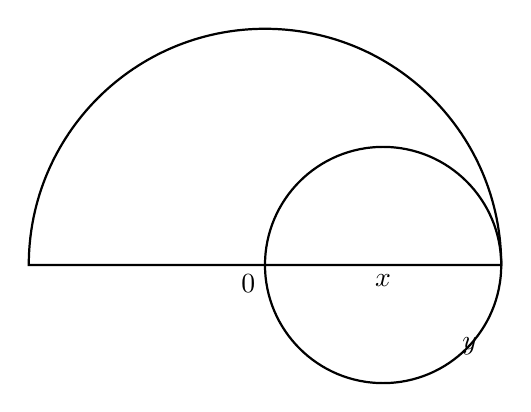
\begin{tikzpicture}
    \draw[thick] (0,0) -- (3,0) arc[start angle=0,end angle=180,radius=3cm] -- cycle;
    \draw[thick] (1.5,0) circle (1.5cm);
    \node[below left] at (0,0) {$0$};
    \node[below] at (1.5,0) {$x$};
    \node[below] at (2.6,-0.8) {$y$};
    \end{tikzpicture}
    $
    Let $y \in B_r(x)$. 
    $
    d(0,y) \leq d(0,x) + d(x,y) \leq \| x \| + r
    $
    $
    \implies B_r(x) \subseteq B_{r + \| x \|}(0).
    $

    \item[(v)] Suppose $S$ is bounded. Then $\exists M \in \mathbb{R}: \forall x \in V \ \| x \| \leq M$
    $
    (\text{Equiv to}\ \exists M \in \mathbb{R}: \forall x \in V) x \in B_M(0).
    $
\end{enumerate}\end{document}